\chapter{Vektorielle Geometrie}


\section{Vektoren}
    \begin{Definition}
        Ein Vektor ist Element eines Vektorraums.
    \end{Definition}\\
    \paragraph{} Vektorräume, wir erinnern uns zurück. Verknüpfungen, inverse Elemente und die dazugehörenden Gesetze, konsequente Definitionen und mathematische Korrektheit, die guten alten Zeiten...\\
    Tatsächlich kann ein Vektor in den meisten Fällen als Verschiebung bezeichnet werden, \textbf{nicht aber als Pfeil oder Strich!}\\

    \subsection{Besondere Vektoren}

        \subsubsection{Der Ortsvektor}

            \paragraph{} Der Vektor von $O$ auf den Punkt $P$, geschrieben als $\vv{OP}$ oder $\vv{o}$.\\
            \paragraph{} Hat $P$ die Koordinaten $(P_1|P_2|...|P_n)$, so besitzt $\vv{o}$ die Darstellung $\left(\begin{array}{c} P_1 \\ P_2 \\ ...\\P_n\end{array}\right)$.

        \subsubsection{Der Nullvektor}

            \paragraph{} Der Vektor mit Wert $\left(\begin{array}{c} 0 \\ 0 \\ ...\\0\end{array}\right)$, er hat keine und alle Richtungen zugleich.
            \begin{Bemerkung}
                Er ist somit das neutrale Element der Vektoraddition.
            \end{Bemerkung}

        \subsubsection{Der Verbindungsvektor}

            \paragraph{} Der Vektor $\vv{AB}$ ist der Vektor, der den Punkt $A$ auf den Punkt $B$ abbildet. Er ist definiert als:\\ $\vv{AB}=\vv{OB}-\vv{OA}$, woraus folgt, dass: \begin{center} $\vv{AB} = \left(\begin{array}{c} b_1 - a_1 \\ b_2 - a_2 \\ ... \\ b_n - a_n \end{array}\right)$. \end{center}

        \subsubsection{Der Gegenvektor}

            \paragraph{} Der Gegenvektor zu $\vv{AB}$ ist $\vv{BA}$, definiert als  $-\vv{AB}$.
            \begin{Bemerkung}
                Er ist somit das inverse Element der Vektoraddition.
            \end{Bemerkung}

    \subsubsection{Der Einheitsvektor}

        \subsubsubsection{Norm eines Vektors}

            \paragraph{} Die Norm eines Vektors ist anschaulich als seine Länge zu interpretieren. Der Betrag, wie sie ebenfalls genannt wird, eines Vektors $\vv{v}$ ist folgendermaßen definiert: $\text{|}\vv{v}\text{|} = \sqrt{\displaystyle\sum_{i=1}^{n}v_{i}^2} ; \vv{v}\in\R^n$.
            \\
            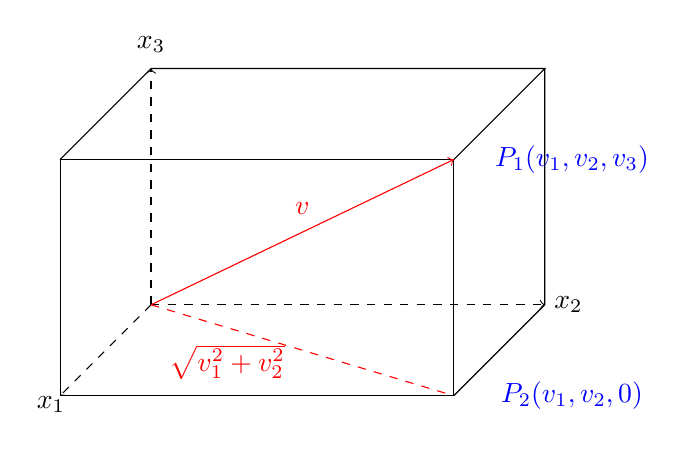
\begin{tikzpicture}
                \draw[dashed, ->] (0,0,0) -- (0,0,3);
                \draw[dashed, ->] (0,0,0) -- (5,0,0);
                \draw[dashed, ->] (0,0,0) -- (0,3,0);
                \draw[dashed, color=red] (0,0,0) -- (5,0,3);
                \draw (0,0,3) -- (5,0,3) -- (5,3,3) -- (0,3,3) -- (0,0,3);
                \draw (0,3,3) -- (0,3,0) -- (5,3,0) -- (5,3,3);
                \draw (5,3,0) -- (5,0,0) -- (5,0,3);
                \draw[->, color=red] (0,0,0) -- (5,3,3);
                \draw (0,0,3.3) node {$x_1$};
                \draw (5.3,0,0) node {$x_2$};
                \draw (0,3.3,0) node {$x_3$};
                \draw (2.5,1.8,1.5) node [color=red]{$\vv{v}$};
                \draw (6.5,3,3) node [color=blue]{$P_1 (v_1, v_2, v_3)$};
                \draw (6.5,0,3) node [color=blue]{$P_2 (v_1, v_2, 0)$};
                \draw (1.7,0,1.9) node [color=red]{$\sqrt{v_1^{2}+v_2^{2}}$};
            \end{tikzpicture}
            \paragraph{} Anhand dieser Graphik lässt sich die Berechnung der Norm eines Vektors $\vv{v}\in\R^3$ verdeutlichen. Für diesen glit: $\text{|}\vv{v}\text{|}=\sqrt{v_1^{2}+v_2^{2}+v_3^{2}}$.
            \paragraph{} Ein Vektor, dessen Norm 1 beträgt wird als normiert oder Einheitsvektor bezeichnet. Für jeden Vektor $\vv{v}\in\R^{3}$ existiert ein Einheitsvektor $\vv{v^{*}}$ , der folgendermaßen definiert wird: $\vv{v^{*}}=\frac{1}{\text{|}\vv{v}\text{|}}*\vv{v}$.

\section{Linearkombination}

    \paragraph{} Vektoren lassen sich allgemein mit der additiven Verknüpfung des Vektorraumes verknüpfen. Diese Verknüpfung zwischen zwei beliebigen Vektoren $\vv{v}$ und $\vv{u}$ erfolgt, wie auch schon im Teil Verbindungsvektor gezeigt wird, wie folgt: $\vv{v}+\vv{u}=\left(\begin{array}{c}{v_1+u_1 \\ v_2+u_2 \\ ... \\ v_n+u_n}\end{array}\right)$.
    \\
    \begin{Definition}
       Eine Familie von Vektoren $\vv{a_1},\vv{a_2},...,\vv{a_n}\in V$ wird als linear abhängig bezeichnet, wenn die Gleichung: \\$r_1\cdot\vv{a_1}+r_2\cdot\vv{a_2}+...+r_n\cdot\vv{a_n}=\vv{0};r_i\in\R$ nicht nur die triviale Lösung $r_1=r_2=...=r_n=0$ besitzt. Existiert nur diese Lösung, ist die Familie linear unabhägig.
    \end{Definition}
    \paragraph{} Anders gesagt, ist eine Familie von Vektoren linear abhängig, wenn sich einzelne Vektoren dieser Familie als Linearkombination von einer beliebigen Anzahl anderer Vektoren der Familie darstellen lassen.
    \begin{Bemerkung}
      Eine linear abhängige Familie \textbf{aus genau zwei} Vektoren wird als kollinear bezeichnet.
      \\
      Eine linear abhängige Familie \textbf{aus genau drei} Vektoren, als komplanar.
    \end{Bemerkung}
\section{Basen und Erzeugendensystem}
    \paragraph{} Eine endliche Anzahl von Vektoren $\vv{a_1},\vv{a_2},...,\vv{a_n}\in V$ heißt Erzeugendensystem, wenn sich \texbf{jeder} Vektor $\vv{v}\in V$ als Linearkombination dieser Vektoren schreiben lässt. Um ein Erzeugendensystem zu bilden benötigt man mindestens die Anzahl Vektoren, die der Anzahl von Dimensionen von $\vv{v}$ entspricht. Wenn man \textbf{genau} diese Anzahl besitzt, spricht man von einer Basis.
    \subsection{Besondere Basen}
        \subsubsection{Orthogonalbasis}
        \paragraph{} Sind die Vektoren der Basis paarweise orthogonal zueinander, so spricht man von einer \textbf{Orthogonalbasis}.
        \subsubsection{Orthonormalbasis}
        \paragraph{} Sind die Vektoren zusätzlich zu dieser Bedingung normiert, wird sie als \textbf{Orthonormalbasis} bezeichnet. Die einfachste und meist benutzte Basis des $\R^3$ besteht aus den drei Vektoren $\vv{e_1}=\left(\begin{array}{c}{1\\0\\0}\end{array}\right),\vv{e_2}=\left(\begin{array}{c}{0\\1\\0}\end{array}\right),\vv{e_3}=\left(\begin{array}{c}{0\\0\\1}\end{array}\right)$. Sie wird als \textbf{Standardbasis} des $\R^3$ bezeichnet. Vektoren wie $\vv{v}=\left(\begin{array}{c}{2\\3\\8}\end{array}\right)$ lassen sich als eine Linearkombination der drei Vektoren der Standardbasis darstellen: $\vv{v}=2\cdot\vv{e_1}+3\cdot\vv{e_2}+8\cdot\vv{e_3}$.
    \subsection{Basistransformation}

        \paragraph{} Bilden die Vektoren $\vv{a_1},\vv{a_2},...,\vv{a_n}$ eine Basis des $n$-dimensionalen Vektorraums $V$ und sei der Vektor $\vv{v}=\left(\begin{array}{c}{v_1\\v_2\\...\\v_n}\end{array}\right);\vv{v}\in V$. Dann gilt wie üblich: $\vv{v}=v_1\cdot\vv{a_1}+v_2\cdot\vv{a_2}+...+v_n\cdot\vv{a_n}$. Sei eine weitere Basis $\vv{b_1},\vv{b_2},...,\vv{b_n}$ des selben Vektorraumes, so besitzt der Vektor $\vv{v}$ andere Koordinaten: $\vv{v}=\left(\begin{array}{c}{v'_1\\v'_2\\...\\v'_n}\end{array}\right)$. Dabei muss gelten: $\vv{v}=v_1\cdot\vv{a_1}+v_2\cdot\vv{a_2}+...+v_n\cdot\vv{a_n}=v'_1\cdot\vv{b_1}+v'_2\cdot\vv{b_2}+...+v'_n\cdot\vv{b_n}$.

        \begin{Bemerkung}
            Um die Koordinaten eines Vektors in einer anderen Basis als der Aktuellen zu bestimmen, löst man diese Gleichung, die sich ergibt.
        \end{Bemerkung}

        \begin{Beispiel}
            Basis 1: Standardbasis des $\R^3$, Basis 2: $\vv{b_1}=\left(\begin{array}{c}{4\\9\\-1}\end{array}\right), \vv{b_2}=\left(\begin{array}{c}{-2\\-2\\8}\end{array}\right), \vv{b_3}=\left(\begin{array}{c}{1\\3\\1}\end{array}\right)$, Vektor $\vv{v}=\left(\begin{array}{c}{-5\\3\\2}\end{array}\right)$ (in der Standardbasis des $\R^3$)
            \\
            $\vv{v}=-5\cdot\vv{a_1}+3\cdot\vv{a_2}+2\cdot\vv{a_3}=r\cdot\vv{b_1}+s\cdot\vv{b_2}+t\cdot\vv{b_3}$
            $\Leftrightarrow \begin{vmatrix}4r & -2s & t & = & -5 \\
                                            9r & -2s & 3t & = & 3 \\
                                            -r & 8s & t & = & 2
                            \end{vmatrix}
             \\
             \\
             \Leftrightarrow \begin{vmatrix}-r & 8s & t & = & 2 \\
                                            0 & 30s & 5t & = & 3 \\
                                            0 & 70s & 12t & = & 21
                             \end{vmatrix}
             \\
             \\
             \Leftrightarrow \begin{vmatrix}-r & 8s & t & = & 2 \\
                                            0 & 30s & 5t & = & 3 \\
                                            0 & 0 & \frac{1}{3}\cdot t & = & 14
                             \end{vmatrix}
             \\
             \\
             \Leftrightarrow \begin{vmatrix}t & = & 99.2 \\
                                            s & = & -6.9 \\
                                            r & = & 42
                             \end{vmatrix}
            \\
            \\
            \mathbb{L}=\{ 42|-6.9|99.2 \}$
            \\
            Daraus lässt sich folgern: $\vv{v}=42\cdot\vv{b_1}-6.9\cdot\vv{b_2}+99.2\cdot\vv{b_3}=\left(\begin{array}{c}{42\\-6.9\\99.2}\end{array}\right)$ (in der anderen Basis).
            \\
            Ich hab keinen Plan, ob meine Berechnungen stimmen, aber es ging vorerst um das Prinzip. Könnte jemand mal bitte nachrechnen?

        \end{Beispiel}


\section{Winkel zwischen Vektoren}
    \subsection{Orientierte Winkel}

        \begin{minipage}{0.5\textwidth}\paragraph{} Wenn man in der Mathematik mit Winkeln arbeitet, werden sie immer im mathematisch positiven Sinn angegeben. Dies bedeutet, dass man von einem Vektor oder Schenkel, der an den Winkel grenzt, ausgeht und über Rotation um den Schnittpunkt \glqq gegen den Uhrzeigersinn \grqq zum anderen gelangt, bis beide übereinanderliegen (wenn man davon ausgeht, dass sich beide schneiden). So ergibt sich $\alpha = \angle ABC = \angle ac = (\vv{BA},\vv{BC}) = \frac{\pi}{3}$
        \end{minipage}
        \begin{minipage}{0.5\textwidth}\paragraph{}
        \definecolor{qqwuqq}{rgb}{0.,0.39215686274509803,0.}
        \definecolor{ududff}{rgb}{0.30196078431372547,0.30196078431372547,1.}
        \begin{tikzpicture}[line cap=round,line join=round,>=triangle 45,x=1.0cm,y=1.0cm]
        \clip(-3.32,-2.22) rectangle (8.28,7.16);
        \draw [shift={(-1.66,1.84)},line width=1.2pt,color=qqwuqq,fill=qqwuqq,fill opacity=0.10000000149011612] (0,0) -- (-22.750976342787634:1.2) arc (-22.750976342787634:35.702202191216706:1.2) -- cycle;
        \draw [shift={(-1.66,1.84)},->,line width=1.2pt,color=qqwuqq] (-22.750976342787634:1.2) arc (-22.750976342787634:35.702202191216706:1.2);
        \draw [line width=1.2pt] (-1.66,1.84)-- (3.6,5.62);
        \draw [line width=1.2pt] (1.0674473317121247,3.8000286908501586) -- (1.057535863562698,3.6081908353598435);
        \draw [line width=1.2pt] (1.0674473317121247,3.8000286908501586) -- (0.8824641364373017,3.8518091646401564);
        \draw [line width=1.2pt] (-1.66,1.84)-- (3.92,-0.5);
        \draw [line width=1.2pt] (1.2406633258194237,0.6235927988499189) -- (1.071990998562399,0.5316708427257207);
        \draw [line width=1.2pt] (1.2406633258194237,0.6235927988499189) -- (1.1880090014376012,0.808329157274279);
        \begin{scriptsize}
        \draw [fill=ududff] (3.92,-0.5) circle (2.5pt);
        \draw[color=ududff] (4.06,-0.13) node {$A$};
        \draw [fill=ududff] (-1.66,1.84) circle (2.5pt);
        \draw[color=ududff] (-1.52,2.21) node {$B$};
        \draw [fill=ududff] (3.6,5.62) circle (2.5pt);
        \draw[color=ududff] (3.74,5.99) node {$C$};
        \draw[color=qqwuqq] (-0.66,1.99) node {$\alpha$};
        \draw[color=black,sloped] (1.2,3.65) node {$c$};
        \draw[color=black,pos=.3,below,sloped] (1.06,0.55) node {$a$};
        \end{scriptsize}
        \end{tikzpicture}
        \end{minipage}

        \\
        \begin{minipage}{0.5\textwidth}\paragraph{} Ein Winkel $\alpha$ wird zudem immer so angegeben, dass $\alpha\in I; I = [-\pi,\pi]$ gilt. Dies bedeutet, dass man nur Winkel zwischen $0°$ und $180°$ erhält, und das in beide \glqq Richtungen\grqq, als im mathematisch positiven und negativen Sinn. Diese Einschränkung kennzeichnet man mit dem Ausdruck \glqq modulo $2\pi$\grqq.
        \end{minipage}
        \begin{minipage}{0.3\textwidth}
        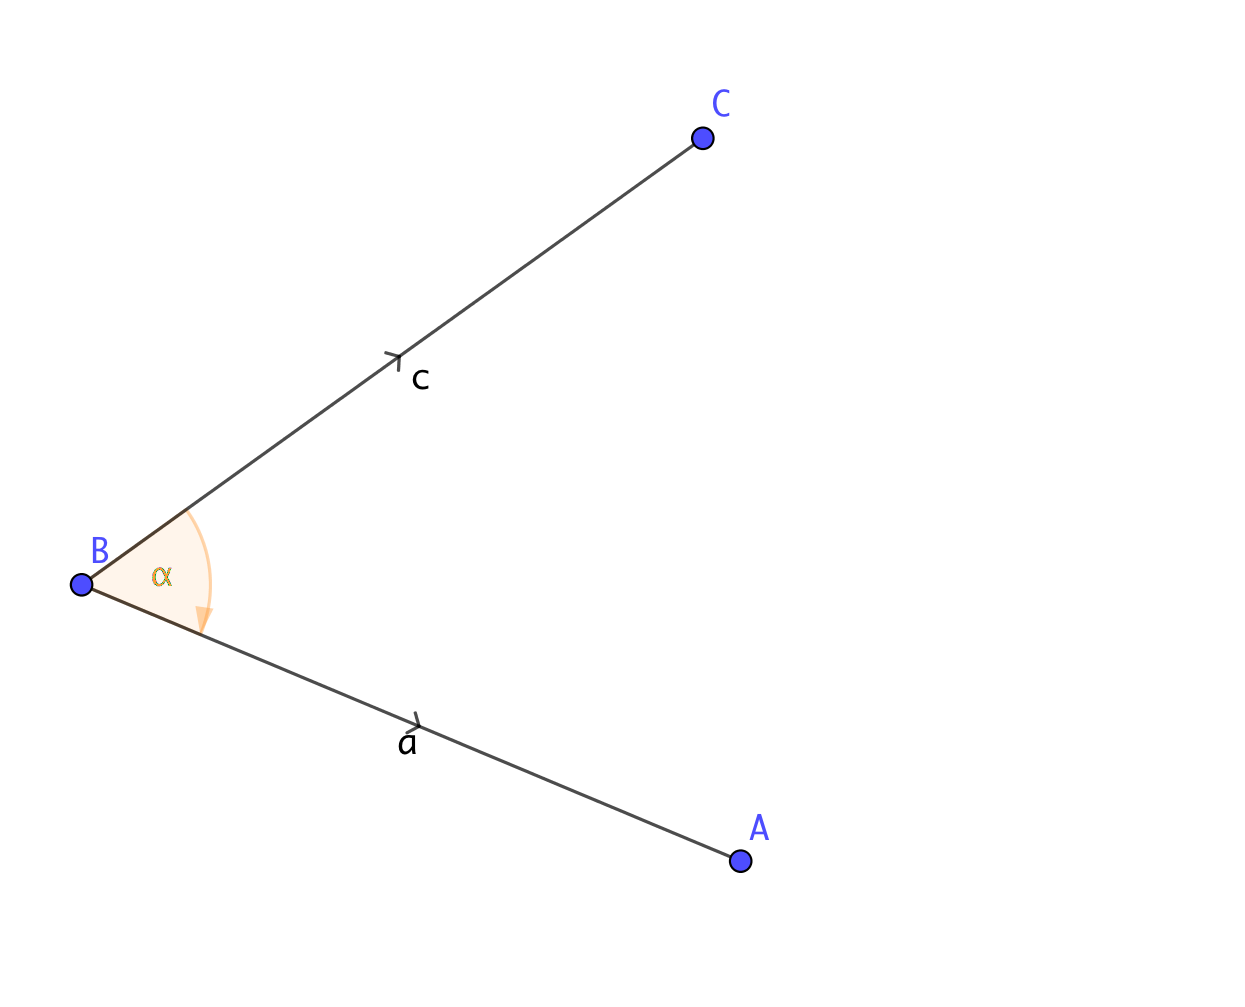
\includegraphics[width=4.7in]{OrientierteWinkel}
        \end{minipage}

    \subsection{}

\section{Geraden}
\section{Ebenen}
\section{Skalarprodukt}
\section{S"atze}

\subsection{Der Satz des Apollinius}
\begin{small}

\begin{Definition}
Gegeben sind: Eine Strecke $[AB]$ und eine positive Zahl $\lambda \in \R^{+} \backslash \{1\}$. Dann ist die Punktmenge

\begin{center}
$M_{A}=\{X| \dfrac{\overline{AX}} {\overline{XB}}=\lambda \}$\\
\end{center}
\\
\\
ein Kreis, den man \textbf{Kreis des Apollinius} nennt.\\
Anschaulich:\\
\\
\\
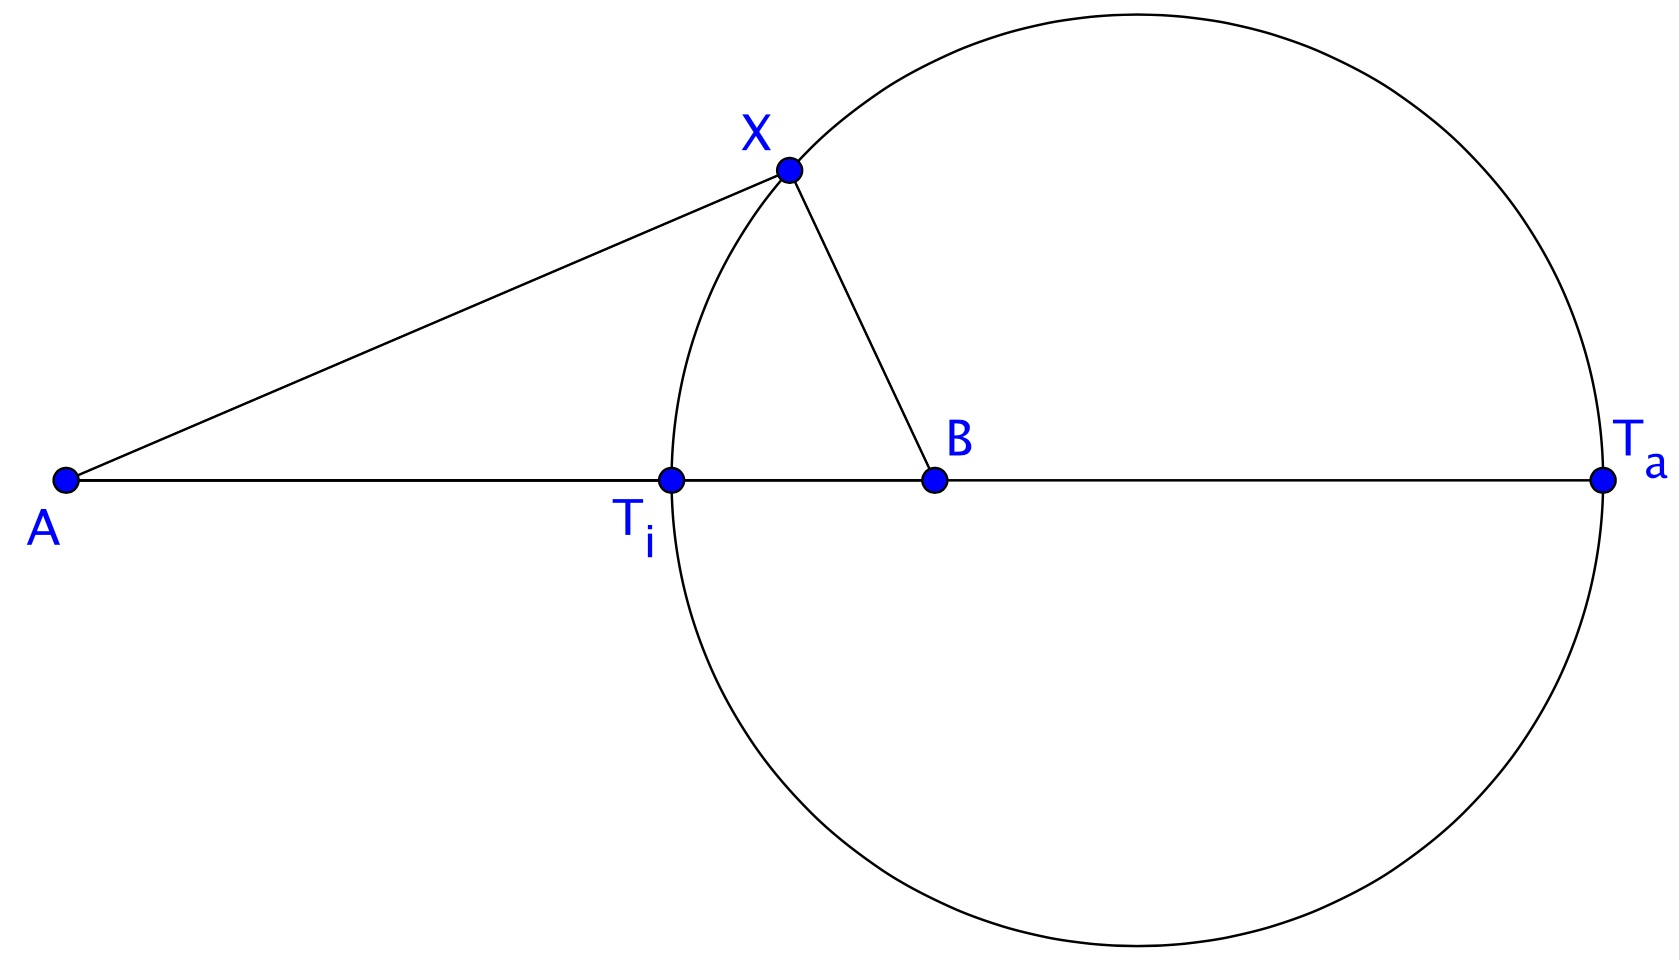
\includegraphics[width=3in]{Apollinus_anschaulich}
\\
Der Satz besagt also, dass alle Punkte $X$ deren Abst"ande zu $A$ ($\overline{AX}$) und zu $B$ ($\overline{XB}$) im Verh"altnis $\lambda$ stehen, auf einem Kreis liegen.\\
\end{Definition}
\newline

\begin{Beweis}
\\
\underline{Beweis:}
Anfangen kann man den den Beweis damit, dass man zwei Punkte sucht, die die Bedingung erf"ullen \textbf{und} auf der Geraden $AB$ liegen. Logisch ist, dass einer dieser Punkte zwischen $A$ und $B$ sein wird, dieser wird \textbf{innerer Teilungspunkt} $T_{i}$ genannt. Der andere Punkt liegt au"serhalb der Strecke $[AB]$ und wird \textbf{"au"serer Teilungspunkt} $T_{a}$ genannt. \\
Im letzten Schritt des Beweises wird man anhand des Skalarprodukts zeigen, dass f"ur alle Punkte $X$, die ebenfalls die Verh"altnisgleichung erf"ullen, die Vektoren $\vv{T_{i}X}$ und $\vv{T_{a}X}$ orthogonal zueinander sind. Somit liegen diese Punkte auf dem Thaleskreis (frz.: Theoreme du triangle rectangle) "uber $T_{i}$ und $T_{a}$, der dann \textbf{Apolliniuskreis} genannt wird.\\
\begin{enumerate}


\item {Um uns die Arbeit so einfach wie m"oglich zu machen, platzieren wir unseren ersten Punkt $A$ auf den Ursprung eines Koordinatensystems und die Strecke $[AB]$ entlang der $x$-Achse . Der Punkt $B$ hat den Abstand $\overline{AB}$ zu $A$, den man $b$ abk"urzt. Gleicherma"sen verf"ahrt man mit den L"angen $\overline{AT_{i}}=t_{i}$ und $\overline{AT_{a}}= t_{a}$, und man f"uhrt den Punkt $X(x|y)$ ein.\\
Hier nochmal ein "Uberblick:\\
\\
\vartriangleright $A(0|0)$ \qquad \vartriangleright $B(b|0)$ \qquad \vartriangleright $T_{i}(t_{i}|0)$ \qquad \vartriangleright $T_{a}(t_{a}|0)$ \qquad \vartriangleright $X(x|y)$\\
\\}

\item {Nun gilt:
\begin{center}
$\dfrac{\overline{AT_{i}}}{\overline{T_{i}B}} = \lambda$ \qquad und \qquad $\dfrac{\overline{AT_{a}}}{\overline{T_{a}B}} = \lambda$ \\
\end{center}
Das benutzt man, um die Koordinaten $t_{i}$ und $t_{a}$ in Abh"angigkeit von $b$ und $\lambda$ auszudr"ucken, denn diese Punkte sind ja durch das Verh"altnis $\lambda$ in der Ebene festgelegt.\\

\begin{minipage}[t]{0.5\textwidth}
\begin{array}{rccl}
&$\dfrac{\overline{AT_{i}}}{\overline{T_{i}B}}$ & $=$ & $\lambda$\\
$\Leftrightarrow & \dfrac{t_{i}}{b-t_{i}} $& $= $& $\lambda$\\
$\Leftrightarrow & $t_{i}$&$=$&$\lambda \cdot b - \lambda \cdot t_{i}$\\
$\Leftrightarrow & \lambda \cdot t_{i} + t_{i}$ &$=$& \lambda \cdot b$\\
$\Leftrightarrow & (\lambda + 1)\cdot t_{i}$&$=$& $\lambda \cdot b$\\
$\Leftrightarrow & t_{i} $&$=$& $ \dfrac {\lambda}{\lambda +1}\cdot b$
\end{array}
\end{minipage}
\begin{minipage}[t]{0.5\textwidth}
\begin{array}{rccl}
&$\dfrac{\overline{AT_{a}}}{\overline{T_{a}B}} $&$ = $&$ \lambda$\\
$\Leftrightarrow $&$ \dfrac{t_{a}}{t_{a}-b} $&$ = $& $\lambda$\\
$\Leftrightarrow & $t_{a}$&$=$&$\lambda \cdot t_{a} - \lambda \cdot b$\\
$\Leftrightarrow & \lambda \cdot t_{a} - t_{a} $&$=$&$\lambda \cdot b$\\
$\Leftrightarrow & (\lambda -1 \cdot )t_{a} $&$=$&$\lambda \cdot b$\\
$\Leftrightarrow & t_{a} $&$=$&$ \dfrac{\lambda}{\lambda -1}\cdot b$\\
\end{array}
\end{minipage}}
\\
\item{ Jetzt wo wir $T_{i}$ und $T_{a}$ in Abh"angigkeit von $b$ und $\lambda$ bestimmt haben, kann man die Vorraussetzung auch noch auf den Punkt $X$ anwenden.\\
\\
\begin{array}{rcccl}
&$\dfrac{\overline{AX}}{\overline{XB}}$ & $=$ & $\lambda$ \\
$\Leftrightarrow & $(\dfrac{\overline{AX}}{\overline{XB}})^2$ & $=$ & \lambda^2$\\
$\Leftrightarrow & $\dfrac{(\overline{AX})^2}{(\overline{XB})^2}$ & $=$ & \lambda^2$\\
$\Leftrightarrow & $\dfrac{x^2+y^2}{(x-b)^2+y^2} $ & $=$ & $\lambda^2$\\
$\Leftrightarrow & $x^2+y^2$ & $=$ & $\lambda^2 \cdtot [(x-b)^2+y^2]$\\
$\Leftrightarrow & $0$ & $=$ & $\lambda^2 \cdot (x-b)^2 +\lambda^2 y^2 -x^2 -y^2$\\
$\Leftrightarrow & $0$ & $=$ & $x^2\cdot \lambda^2 - 2bx\cdot \lambda^2 +b^2\cdot \lambda^2 +y^2\cdot \lambda^2 -x^2-y^2 $ &\textcolor{red}{(1)}\\
\\
\end{array}
}



\item{
Bevor man zum Ende kommt, kann man noch die Ergebnisse aus 2) benutzen, um $t_{i}$ und $t_{a}$ miteinander zu verrechnen, denn diesen Zusammenhang braucht man gleich.\\
\begin{center}
\begin{array} {rccccccl}
$t_{i} + t_{a} $ & $=$ & $\dfrac {\lambda}{\lambda +1}\cdot b + $\dfrac {\lambda}{\lambda -1}\cdot b  $ &$=$& $(\dfrac{\lambda}{\lambda+1} + \dfrac{\lambda}{\lambda-1})\cdot b$ & $=$ & $\dfrac{\lambda^2}{\lambda^2 -1}\cdot 2b$ \qquad \textcolor{red}{(2)}\\
\end{array}
\\
\begin{array} {rcccccl}
$t_{i} \cdot t_{a} $ & $=$ & $\dfrac {\lambda}{\lambda +1}\cdot b \cdot $\dfrac {\lambda}{\lambda +1}\cdot b $ & $=$ & $\dfrac{\lambda^2}{\lambda^2 -1}\cdot b^2$ \qquad \textcolor{red}{(3)}\\ \\
\end{array}
\end{center}
}

\item{
Nun kommt der finale Schritt. Man bildet die Vektoren $\vv{T_{i}X} = \left(\begin{array}{c} x-t_{i} \\ y \end{array}\right)$ und $\vv{T_{a}X} = \left(\begin{array}{c} x-t_{a} \\ y \end{array}\right)$ und berechnet deren Skalarprodukt. $\ast$ TROMMELWIRBEL$\ast$ \\
\\
\begin{center}
\begin{array}{rccl}
$\vv{T_{i}X} \cdot \vv{T_{a}X}$ &$=$& $(x-t_{i})\cdot (x-t_{a}) +y^2$\\
& $=$ & $x^2 -(t_{i} +t_{a})x + t_{i}\cdot t_{a} + y^2$ & $Benutze (2) und (3) \\
& $=$ & $x^2 - \dfrac{\lambda^2}{\lambda^2 - 1} \cdot 2bx + \dfrac{\lambda^2}{\lambda^2 - 1} \cdot b^2 +y^2$\\
& $=$ & $\dfrac{x^2 \cdot (\lambda^2 -1) - 2bx\cdot \lambda^2 + b^2\cdot \lambda^2 + y^2 \cdot (\lambda^2 -1)}{\lambda^2 -1}$\\
& $=$ & $\dfrac{x^2 \cdot \lambda^2 - 2bx\cdot \lambda^2 b^2\cdot \lambda^2 +y^2\cdot \lambda^2 -x^2 -y^2} {\lambda^2 -1}$ &  $Benutze (1) \\
& $=$ & $0$\\
\\
\end{array}
\end{center}
}

Damit hat man bewiesen, dass f"ur alle Punkte $X$ die Vektoren $\vv{T_{i}X}$ und $\vv{T_{a}X}$ orthogonal zueinander sind, weshalb sie auf dem Thaleskreis "uber $T_{i}$ und $T_{a}$ liegen m"ussen.\\ \\
\end{enumerate}
\end{Beweis}


Die Figur und die Zusammenh"ange, die man durch den Satz des Apollinius erhalten hat, kann man benutzen, um ein wenig mit Winkeln zu spielen: \\
\\
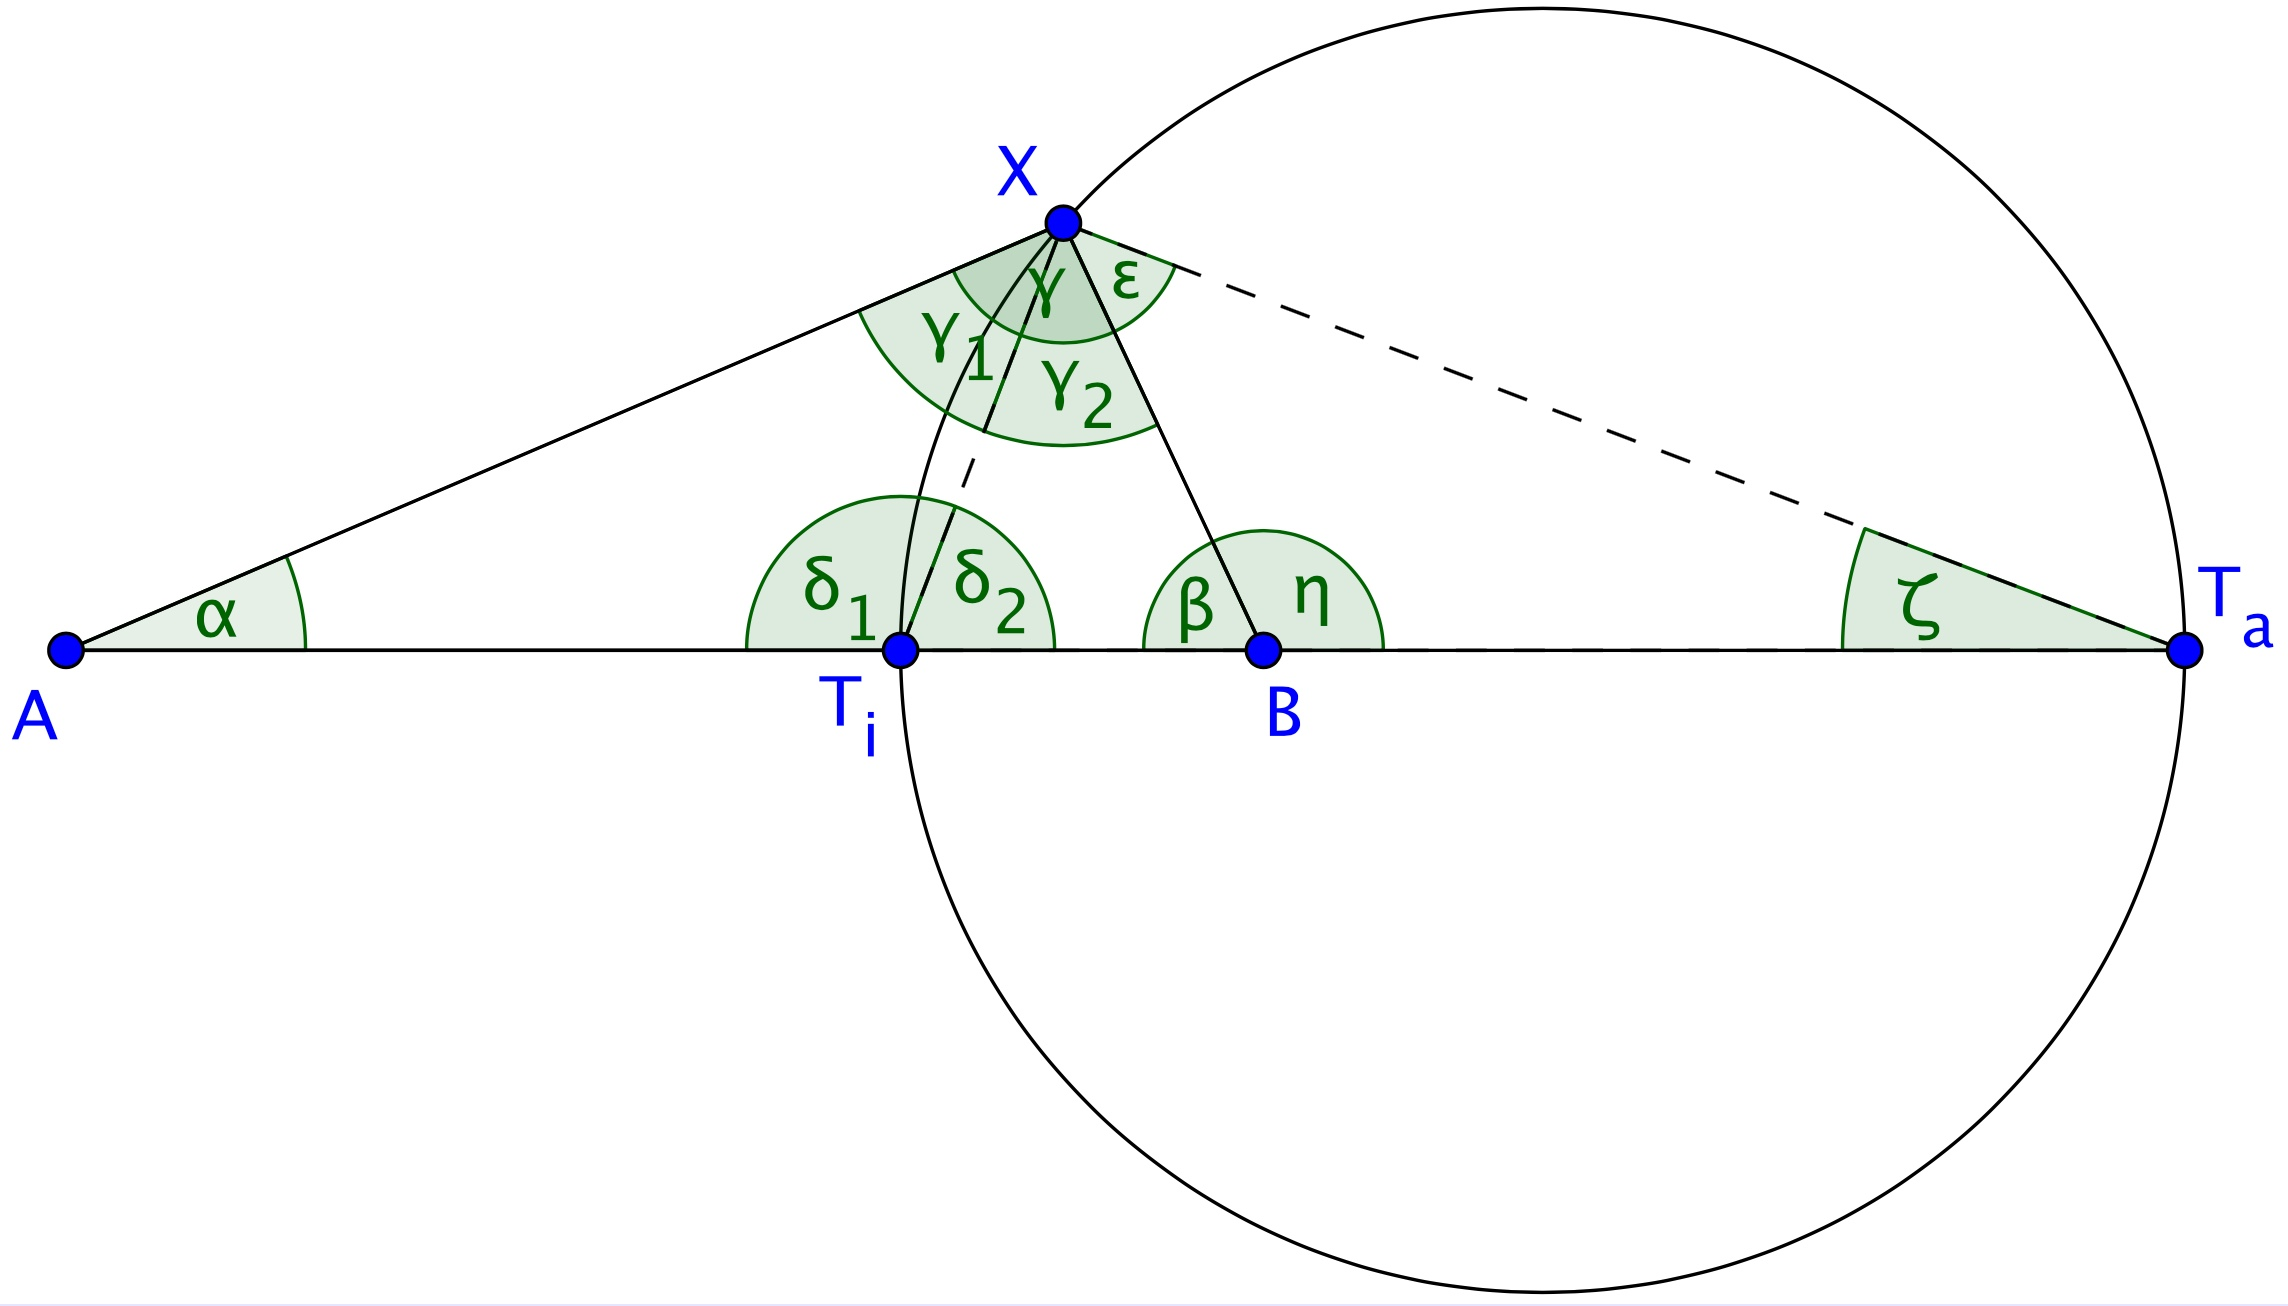
\includegraphics[width=5in]{Apollinius_Winkel}\\
\\
\begin{mdframed}
Auf dieser Skizze sind 10 Winkel gekennzeichnet, zu welchen sich eine ganze Reihe von Beziehungen aufstellen l"asst:\\
\\
\begin{array}{rcccl}
$\vartriangleright \alpha + \beta + \gamma = 180 $ & $\vartriangleright \beta + \gamma_{2} + \delta_{2} = \ang{180} $ & $\vartriangleright \delta_{1} + \delta_{2} = \ang{180} $ & $\vartriangleright \alpha + \gamma + \epsilon + \zeta = \ang{180} $ &$\vartriangleright \epsilon + \zeta + \eta = \ang{180}$\\
$\vartriangleright \aplha + \gamma_{1} + \delta_{1} = \ang{180} $ & $\vartriangleright \gamma_{1} + \gamma_{2} = \gamma $ & $\vartriangleright \gamma_{2} + \epsilon = \ang{90} $ & $\vartriangleright \beta + \eta = \ang{180} $ &$\vartriangleright \gamma_{2} + \delta_{2} + \epsilon + \zeta = \ang{180}$\\
\\
\end{array}
\\
Hiermit bekommt man ein zehndimensionales Gleichungssystem mit dem sich $\gamma_{1} = \gamma_{2}$ zeigen l"asst. Dies bedeutet dass die Gerade $T_{i}X$ auch noch die Winkelhalbierende des Winkels $\gamma = \angle AXB$ ist:
\\
\end{mdframed}
\begin{Definition}
Eine Innenwinkelhalbierende eines Dreiecks teilt die gegen"uberliegende Seite im Verh"altnis der Anliegenden Seiten. \qquad $\gamma_{1}=\gamma_{2} \Rightarrow \overline{AT_{i}}:\overline{T_{i}B}=\overline{AX}:\overline{XB}$
\end{Definition}
 \begin{center}
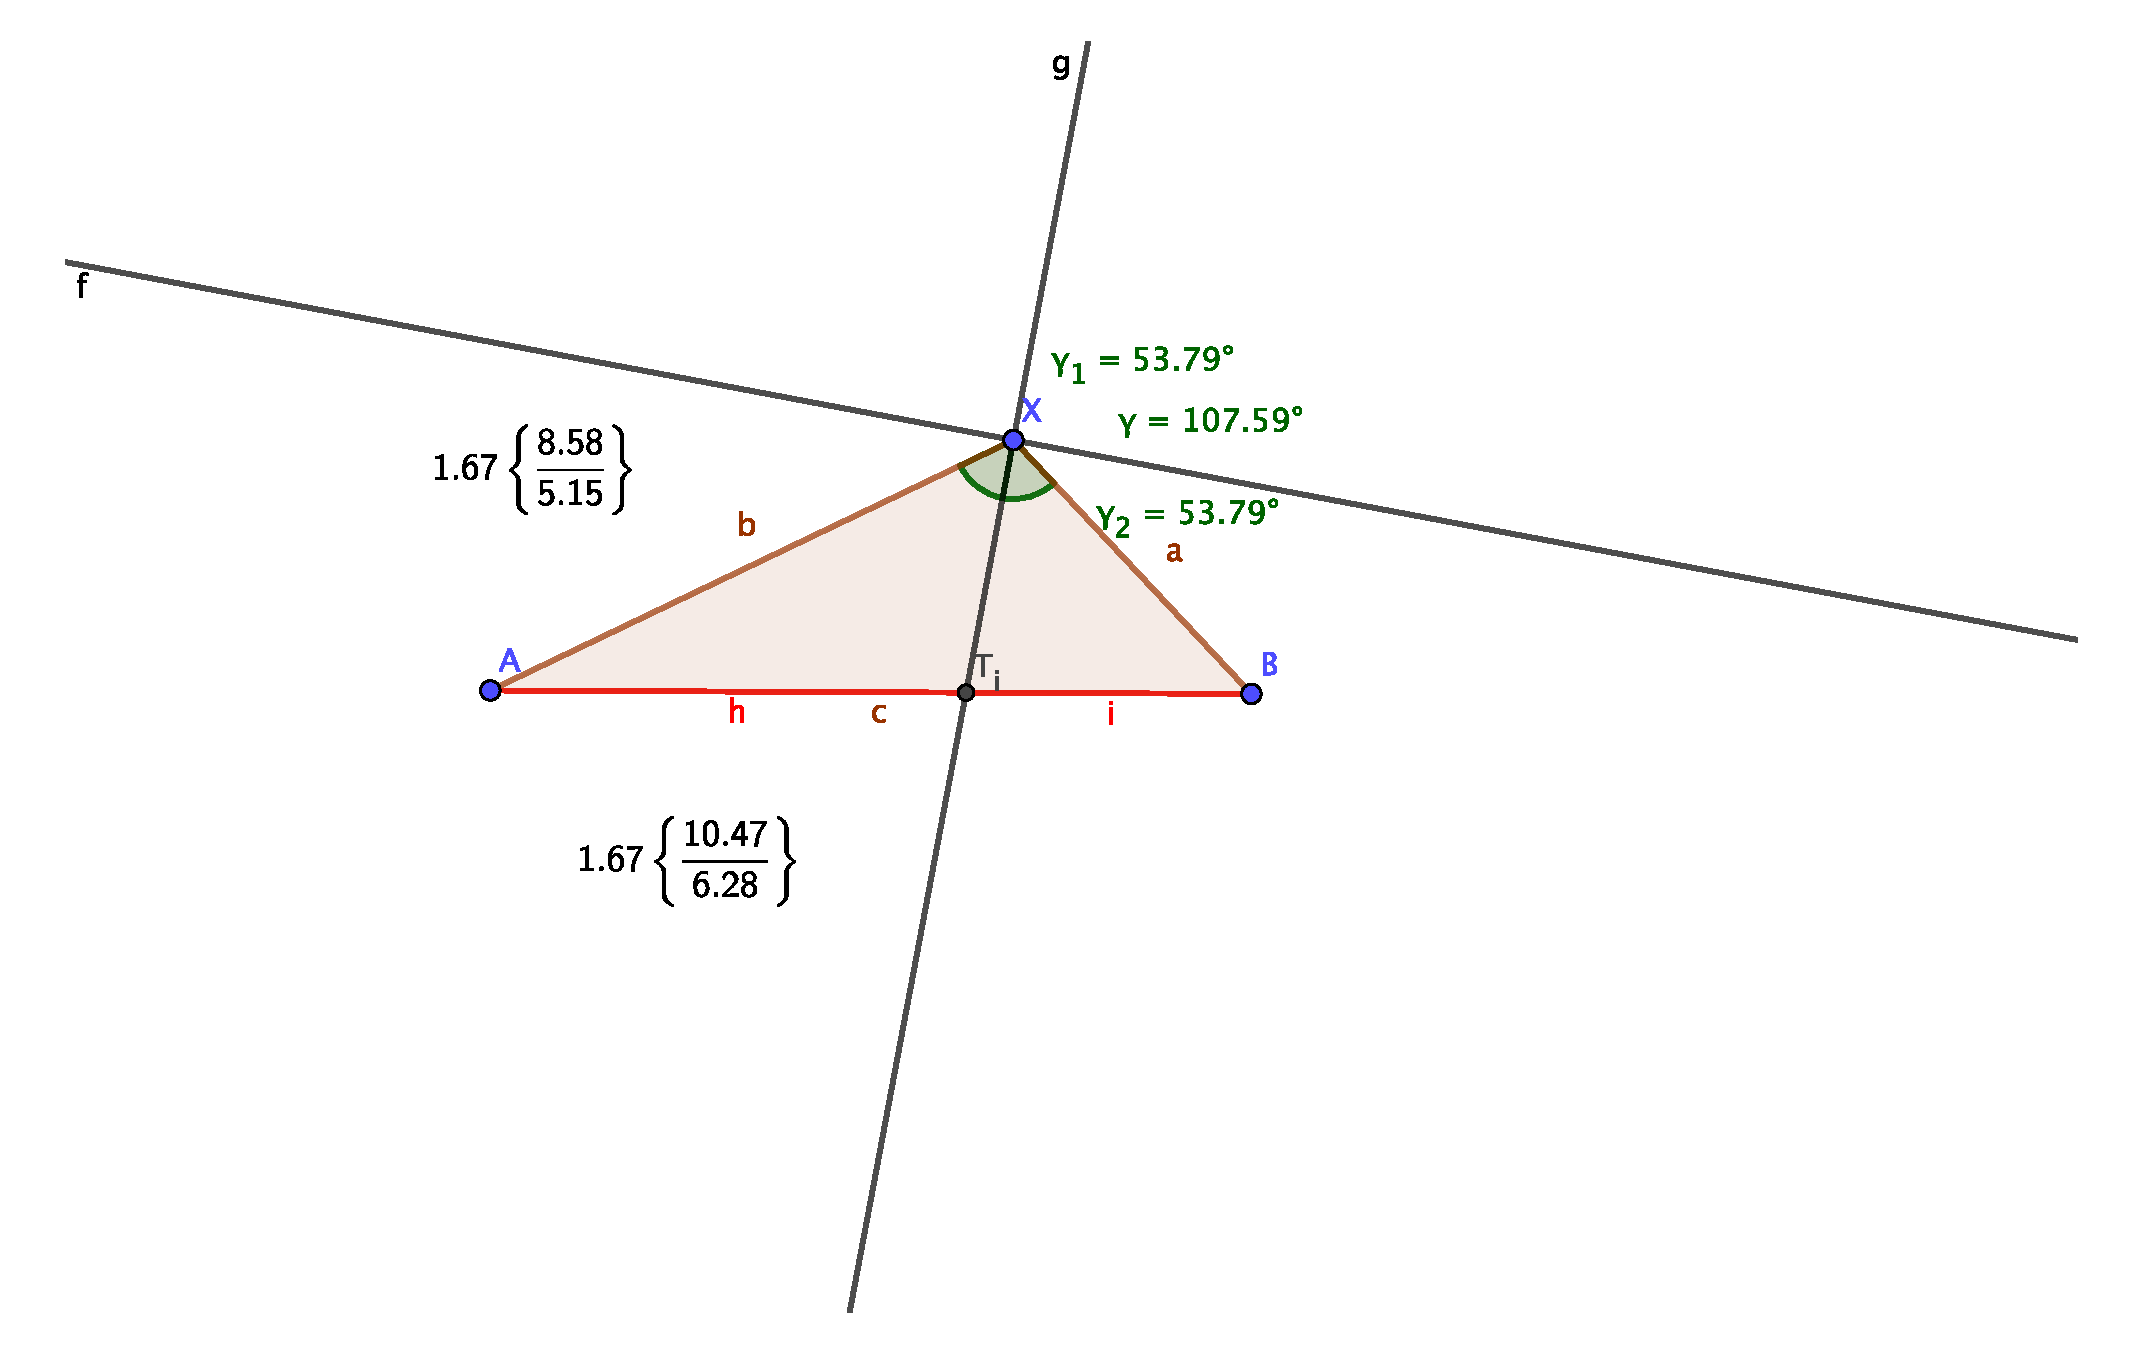
\includegraphics[width=4.7in]{Apollinus_Winkelhalbierende_Bild}
\end{center}
\end{small}
\begin{tiny}
  Quelle : Tobias Rave, 06.03.18, Skript 1ere SBC S.68-71
\end{tiny}
